\documentclass[10pt,a4paper,twoside]{llncs}
\usepackage[left=3cm,right=3cm,top=2.5cm,bottom=2.5cm]{geometry}
\pagestyle{plain}
\setcounter{secnumdepth}{3}%to set numbering over subsubsections

\usepackage[latin1]{inputenc}

\usepackage{amsmath,amsfonts,amssymb}
\usepackage{graphicx}
\usepackage{pstricks}    %for embedding pspicture.
\usepackage{epsfig}
\usepackage{algorithmic,algorithm}
\usepackage[colorlinks=true,linkcolor=blue,urlcolor=blue,citecolor=blue]{hyperref}


%%%%%%%%%%%%%%%%%%%%%%%%%%% VERSIONES %%%%%%%%%%%%%%%%%%%%%%%%%%%%%%%%%%%
%\usepackage{gitinfo}
%\newcommand{\version}{github.Papers: \gitCommitterDate\;(revision \gitAbbrevHash) } %!!fixme!!
\newcommand{\todo}[1]{\texttt{\color{red}TODO:} ``\emph{#1}''}
\newcommand{\fixme}[1]{\texttt{\color{red}FIXME:} ``\emph{#1}''}
\newcommand{\ok}[1]{``#1'' [\texttt{\color{green}OK}]}
%%%%%%%%%%%%%%%%%%%%%%%%%%%%%%%%%%%%%%%%%%%%%%%%%%%%%%%%%%%%%%%%%%%%%%%%%

\newcommand{\tango}{\textsc{Tango}}
\newcommand{\atk}{\textsc{Atk}}
\newcommand{\sardana}{\textsc{Sardana}}
\newcommand{\taurus}{\textsc{Taurus}}
\newcommand{\mambo}{\textsc{Mambo}}

\newcommand{\corba}{\textsc{Corba}}
\newcommand{\omniorb}{\textsc{omniORB}}
\newcommand{\zmq}{\textsc{$\varnothing$mq}}
\newcommand{\mysql}{\textsc{MySql}}



%opening
\title{Agent security in Distributed Control Systems: \\The case of \tango}
\author{Sergi Blanch-Torn\'e\inst{1}}%, Fernando Cores Prado\inst{2}, Ramiro Moreno Chiral\inst{3}, Francesc Seb\'e Feixa\inst{3}}
 \institute{
 Escola Polit\`ecnica Superior, Universitat de Lleida. Spain.\\
 \email{\tt sblanch@alumnes.udl.es}
%  \and
%  Dept. d'Inform\`atica i Enginyeria Industrial. Universitat de Lleida. Spain.\\
%  \email{\tt fcores@diei.udl.cat}
%  \and 
%  Departament de Matem\`atica. Universitat de Lleida. Spain.\\
%  \email{\tt \{ramiro,fsebe\}@matematica.udl.es}
 }

\begin{document}

\maketitle
\begin{center}
 {\tt DRAFT}\\
 \today\\
 %\version
\end{center}

\begin{abstract}\footnote{Partially supported by grants MTM2010-21580-C02-01 (Spanish Ministerio de Ciencia e Innovaci\'on), 2009SGR-442 (Generalitat de Catalunya).}
 
    Distributed Control Systems are a solution that mixes two concepts: Industrial Control and Distributed Systems. Nowadays this type of solution is widely spread in disseminated resources by networks that can be open accessed or, in the best case, only protected by firewalls. The problems that an attack to this systems can cause can be quantified easily when keystone industries are targeted like energy grids or one can imagine the effects on other like traffic lights. Too often, during the developments, the security is forgotten in favour of time schedule restrictions.

    \tango\, is an example of this Distributed Control Systems where by its isolated environment inside an institution (firewalled cases) has helped to avoid the security issues. But this is a defect that blocks this systems to arrive to a new horizon of industries. Recently voices have raised the problem and a request has arrived to introduce this goal to the system core.

    As in the past has happen with the world wide protocols, like web, e-mail and others, it is a requirement for exposed to attacks systems to have security protocols to cover the security over the different levels of the communication.

{\bf Keywords:} Cryptography\footnote{This big keyword includes proposals over \emph{Public key}, \emph{Elliptic Curves}, \emph{Symmetric algorithms}, \emph{stream cyphers}, \emph{secret sharing} and also \emph{Homomorphic encryption} for databases.}, Distributed Control Systems, Cryptography Engineering.

\end{abstract}

%%%%%%%%%%%%%%%%%%%%%%%
\section{Introduction}\label{sec:introduction}

\tango\, is a software tool supported by the \emph{Consortium}\footnote{see \href{https://www.tango-controls.org/}{tango-controls.org} for further information about the consortium.} where 8 of the member institutions are synchrotrons\footnote{Synchrotron is a circular particle accelerator design to generate electromagnetic radiation (specially in the region of the X-rays but not only). This light is used in scientific experiments} and the ninth is a neutron source\footnote{Neutron sources are scientific facilities with nuclear reactors or particle accelerators designed to emit neutrons for experimental studies}. Apart from this institutions there are other projects that uses \tango\, to control the research facility and recently the industry have shown interest to use it in their process. But this industry have pointed a very important feature forgotten in this system, the security. An not concerning only the classical IT environmental security, that is a institution/user choice, the feature is about the use 
of cryptology to mathematically protect the 
system.

A goal of ensure \tango\, must produce an outcome as similar as the \emph{TLS} is for the web navigation or e-mail, but not only. The final goal to provide security must be involve the other levels of the Open System Interconnection model (the OSI layers) by provide end-to-end agent authentication and encryption. Event than a migration environment should allow to coexist with non secured access, the setup of the system must provide a complete transparent security. Concepts like the certificates shall be integrated to not increase the current complexity of a \tango\, installation.

The instances running of \tango\, are in a very specialized situation, but the scientific facilities may not be so different than industry applications. \tango\, runs over different architectures and operating systems, having the computing sources of a very big computer with small embedded systems in the same network. When security is introduced, it must not ``disturb'' or it's easily deactivated. Then the solutions shall work fine in the smaller case, and \emph{Elliptic curves}, \emph{lightweight symmetrics} and \emph{stream cyphers} are the best candidates on this business.

\tango\, is a Free Software implementation, divided in 2 parts (as will be explained in section \ref{sec:concepts}). The core is distributed under \emph{LGPLv3} license and the device servers distributed by the \emph{Consortium} are licensed under \emph{GPLv3}. There are other satellite tools in \tango\, that helps to cover more area and extend the usage. This tools are also distributed under Free Software licenses and they are \atk, \sardana\footnote{See \href{https://www.sardana-controls.org/}{sardana-controls.org} for further information about this collaboration.}, \taurus (to help on the SCADA behaviour) and \mambo (that covers the feature of the data archiving). The auxiliary tools used inside the \tango\, implementation are also Free Software as it is the \omniorb \cite{omniORB41} and \zmq \cite{zmq32}.

It is very important goal to have the \tango\, implementation as Free Software, as this paper cryptography outcomes must be to have public access with auditable algorithms and sources.

\begin{itemize}
    \item \todo{Structure of this paper}
\end{itemize}


%%%%%%%%%%%%%%%%%%
\section{Concepts}\label{sec:concepts}

%%%%%%%%%%%
\subsection{Industrial control}\label{sec:IndCtrl}

Largely used in the industry, a \emph{Distributed Control system} is a particular case of an \emph{Industrial Control System} and is a particular case of \emph{distributed computer network}. Lets start from the industrial side for the definitions.

\begin{definition}[\href{http://en.wikipedia.org/wiki/Industrial_Control_System}{Wikipedia (en)}]\label{def:ICS}
    \emph{Industrial Control System} (short for ICS) is a general term that encompasses several types of control systems used in industrial production, including \emph{Supervisory Control And Data Acquisition} (short fro SCADA) systems, \emph{Distributed Control Systems} (short for DCS), and other smaller control system configurations such as \emph{Programmable Logic Controllers} (short for PLC) often found in the industrial sectors and critical infrastructures.
\end{definition}

In this definition \ref{def:ICS} are nested 3 concepts that must de also defined, and lets start from the smaller and then continues for the next little bigger.

\begin{definition}[\href{https://en.wikipedia.org/wiki/Programmable_logic_controller}{Wikipedia (en)}]\label{def:PLC}
    A \emph{Programmable Logic Controller} (PLC) is a digital computer used for automation of electromechanical processes, such as control of machinery on factory assembly lines, amusement rides, or light fixtures.
\end{definition}

With PLCs a production line can be controlled and monitored. This systems, even they are thought for local uses, often have telephony \emph{sim} cards and are exposed throw insecure environments. Above those PLCs, the common is to have \emph{Graphical User Interfaces} (short for GUI), and them are also the next level in the ICS.

\begin{definition}[\href{http://es.wikipedia.org/wiki/SCADA}{Wikipedia (es)}]\label{def:SCADA}
    A \emph{Supervisory Control And Data Acquisition} (SCADA) is a computer software to control and supervise industrial process remotely.
\end{definition}

By this definition of SCADA, many more computing elements can be introduced. As mention before, below SCADAs can be one or many PLCs, but also other computers with other very specific tasks, like specific measurement cards plugged or FPGAs\footnote{FPGA is the short for Field-Programmable Gate Array even is widely used in Controls, here is not have its definition because it is not considered an element of an ICS, but can be comparable to a PLC}. Once here a higher level abstraction can be found when goes to a larger scale:

\begin{definition}[\href{http://en.wikipedia.org/wiki/Distributed_control_system}{Wikipedia (en)}]\label{def:DCS}
    A \emph{Distributed Control System} (DCS) is the computer software for a manufacturing system, process or any kind of dynamic system, in which the controller elements are not central in location (like the brain) but are distributed throughout the system with each component sub-system controlled by one or more controllers.
\end{definition}

%%%%%%%%%%%
\subsection{Distributed systems}\label{sec:DistrSys}

From the \emph{Distributed Control System} definition (\ref{def:DCS}) has been used introduced the concept of a non-centralized system over a network. The concept of the distributed comes from the time when computer networks becomes more and more common and the idea of one processing unit with peripherals become expired. Continuing with the view of the industrial control systems, a PLC is what can be sawn more similar to a single \emph{personal computer}, but with the networks born the idea of many pieces doing related and/or independent tasks but coordinated. From this concepts emerges the definition of a \emph{distributed system}:

\begin{definition}[Tanenbaum \cite{TanenbaumDistr}]\label{def:distributedSystem}
    A \emph{distributed system} is a collection of independent computers that appears to its users as a single coherent system.
\end{definition}

Every single element, called an \emph{agent} of a distributed system is independent of all the others, but its meaning comes from the interaction with those others (and obviously some of them with the user). This independence is what gives one of the most special features to a distributed system: the scalability. Because there is no central point, neither the agents depends hardly one each other, the growing number of agents depends only on the infrastructure capacity. Perhaps more cpu can be required, perhaps more bandwidth, but the number of agents has virtually no limit.

Once a system likes to receive the \emph{tag} of distributed some conditions must be complained. Continuing with the Tanenbaum's explanations, there are several \emph{transparencies} that a candidate for distributed should complain. They are refereed to facts that shall be hide to the user of the system. But every rule can have exceptions, then one can define degrees on this transparencies complain. Not all the distributed systems respect all this transparencies and neither they are complained in the same extension.

\begin{table}[h]
    \begin{center}
        \begin{tabular}{|l|l|}
            \hline
            Access & Hide differences in data representation and how a resource is accessed \\ \hline
            Location & Hide where a resource is located \\ \hline
            Migration & Hide that a resource may move to another location \\ \hline
            Relocation & Hide that a resource may be moved to another location while in use \\ \hline
            Replication & Hide that a resource is replicated \\ \hline
            Concurrency & Hide that a resource may be shared by several competitive users \\ \hline
            Failure & Hide a faulure and recovery of a resource \\ \hline
            Persistence & Hide whether a (software) resource is in memory or on disk \\ \hline
        \end{tabular}
        \caption{Transparencies in distributed systems from \cite{TanenbaumDistr}.}\label{tab:transparencies}
    \end{center}
\end{table}

In table \ref{tab:transparencies} are listed 8 transparencies that a system should complain to be called distributed, but as was said before not all the distributed system follows all of them neither in the same degree. Depending on the requirements of a distributed system those transparencies will need more or less degree of presence. It is not the same a mobile agent system than a DCS. Specifically, in the case of DCS in the industry, a highly specialized hardware would be only controlled from an specific computer that has the precise card plugged. This happens most of the time with \tango, but it does not mean that other agents can be moved from one machine to another, when they do not have requirements like the mention before (for example a cpu intensive processes).

Although the first idea of transparency seems broken by hardware restrictions (one may think in the \emph{location} transparency), this can be wrong. Imagine what would happen if this specialized hardware fails. If the agent can be moved to new location (autonomously) and from there report this failure by itself, the consistency of the system will be greater that to realize of this failure because the agent is not available.

Detailed description on \tango's transparencies will be set up in section \ref{sec:characteristics}

What allows all this agents in a distributed system to be relocated, replicated, and so on with the transparencies is what gives coherence to the system, and this receives the name of \emph{middleware}.

\begin{definition}\label{def:middleware}
    The \emph{middleware} is what supports heterogeneous computers and networks while offering a single system view.
\end{definition}

The middleware is nothing by itself, it is nothing \emph{tangible} in the system in the meaning that the user can not interact with. The middleware is the environment where the agents live, is what stablish the rules that all the agents will follow.

%%%%%%%%%%%
\subsection{Information security}\label{sec:InfoSec}

At this point where is clear what is a Distributed Control System, it is time to define the concept of the \emph{information security}. 

\begin{definition}\label{def:infosec}
    \emph{Information security} is the protection provided to the information in order to minimize the risk that it becomes compromised.
\end{definition}

By this definition \ref{def:infosec} many risks has to be consider like unauthorized access, any modification and also the destruction of the information to be protected. Following this risks the principles of the information security are listed in the table \ref{tab:infosec}. There are the $5$ basics and well know, and has been added a sixth principle about the auditory and a seventh about collateral damages.

\begin{table}[h]
    \begin{center}
        \begin{tabular}{|l|l|}
            \hline
            Confidentiality & Information must be disclosed only to the authorized. \\
            Integrity & Only authorized can set in the system and no one else can modify. \\
            Availability & Information must be accessible for those who are authorized. \\
            Authenticity & Information must only be emitted by the authorized. \\
            Non-repudiation & Forbid validity changes on the information emitters. \\
            \hline
            Auditory & Trace who access where (extremely useful for a security breach analysis). \\
            Third-party & protection to averting damage. \\
            \hline
        \end{tabular}
        \caption{Basic principles of the information security plus extra non-basic objectives.}\label{tab:infosec}
    \end{center}
\end{table}

These last elements about auditory and damage control, are like many other things in security, they are double-edge swords, specially in the auditory case. Always depends on the moment to install an specific system, to device if those principles clashes with privacy. Perhaps that is why they are not \emph{basic}s. Privacy is not against security neither the other way around, but the difference in this auditory principle is who does it and under which circumstances. When is the same the owner who audits itself, with transparency with the users, in order to find if someone is acting improperly, this can be a good tool. But this tool can be also used to spy the behaving of the users.

Further than secure the information itself there is an environment, where the code runs, to be secured. In a distributed system besides the fact of provide the basic principles of the information security, one have to step in the trustiness of the machine where this code is running. From the example of the multi-user machines, where one had to be aware of the other users, in a distributed system there are other agents (perhaps with the same user identification and permissions) running in parallel. The security in the agents communication is not only a matter of networking (the channel), many other layers are involved.

\subsection{Security engineering}\label{sec:SecurityEngineering}

Develop security engineering is a multi-disciplinary field. It is not only a matter of knowing the mathematics behind the cryptology, it also requires a knowledge on networking and hardware behaviour, and very often the psychology to understand how the things applies in practice. It is use less to implement de hardest cryptosystem if this implementation is revealing information in a side channel, or to have the strongest password policy that forces the users to write them on papers because is not humanly possible to remember.

This field makes feel like a bad guy. Everyday training is required and the best way is to think over all the aspects of the live, from the insignificant to transcendent. How to protect a pet shop if you do not allow yourself to think how on steal it? You do not have to steal it but is not impure to think how one that likes to do it can behave as.

In the book ``\emph{Security engineering \cite{SecEngRossAnderson}}'' three\footnote{There is a fourth scenario in the book, but is more a corollary of the previous.} scenarios are highlighted: A \emph{bank}, a \emph{military base} and a \emph{hospital}. Why this three and not others? Probably because with them all the critical assurance requirements are covered. The fundamental on each scenario is the point of view, and any new scenario can be described in terms of different degrees of the characteristics on those highlighted. Any new scenario can use this to define which is the current protection problem on it.

\paragraph{Inside a bank:} In this case what must be clear is the goal of the security: protect information and avoid deceptive transactions. Then the information and the capacity to do these things must be uniquely in the hands of the stuff. But even if there is trust with staff, is a good procedure to dilute the authorizations when the operation has some degree of unusual or dangerousness. To any operation, a degree (or degrees) of different risks can be tabulated. With this information, a single operation can require some level on the person who is doing or even require the approval from more than one person. This also includes current web applications systems where the staff are not directly involved, but the client gets some staff roles.

Another situation described in this kind of scenarios is the monitoring of activity patterns. There are also degrees on privacy invasion, or decay in a need to monitor the one who is monitoring. It is not necessary to go to much in the detail, on the opposite, with enough abstraction, anomalies can be raised and detect, for example, when in one office there is a robbery.

\paragraph{Looking on a military base:} This scenario is an example on where complex systems interact with countermeasures (and often \emph{countercountermeasures} and so on). The desired image from this kind of places is like if it has a dome that looks transparent when it really like to not show anything at all. Not going to the field of the \emph{steganography}\footnote{Steganography from wikipedia: ``the art and science of writing hidden messages in such a way that no one (...) suspects the existence of the message''}, the purpose of security is to distinguish between \emph{friend or enemy} (FoE). The keystone on this scenario is the trust on the incoming information (assuming your own computer is not compromised).

Another characteristic of this kind of scenario to highlight, is a extreme trust in the chain of command, but together with an also extreme requirement of solutions in case of a \emph{head-cut} situation.

\paragraph{A day in a hospital:} A completely different scenario than the previous is what happens with patients records. The access to the information has to be granted to some specific staff in the precise moment that they need to, but this can expire in a while. When some one is receiving treatment, the staff should have access to all the available information, but not when the treatment is done. Later on time, the information should be still available but under an anonymised format to allow medical research without compromise the privacy.

Should not lose sight that an scenario like a hospital is a place where new people is coming in and out quickly, where the staff has to drop what they are doing to run into an emergency when the less priority is a simple act of locking a computer.

In all this case the main issue are the not understanding of security from the heads and administrators. When security measures are understood as arising from cowardice. When security is rejected by considering it as simple paranoia.

% \begin{itemize}
%     \item \todo{Practical paranoia \cite{PractCryptoSchneier}}
%     \begin{itemize}
%         \item Identify threads
%         \item Evaluate attack capabilities
%     \end{itemize}
% \end{itemize}

In security engineering there is an important concept, introduced in \cite{PractCryptoSchneier} under the name of \emph{practical paranoia}. There are security decisions during a distributed system design and implementation, but there are also other decisions related with the time when this system is placed somewhere, put in practice. Then is the moment to respond two extremely basic questions: 

\begin{enumerate}
    \item How much value has the information?
    \item How much resources has the attacker?
\end{enumerate}

These questions have reference to define how high should be the wall you build using cryptology. There must be a balance between how important is the information and the cost of protect this information. Often that is not easy to answer, from one side because the value of the information can be objectivated but with a subjective component, and the resources from the attacker are estimated (any of the potential attackers should not show the real potential), and the attacker's motivation must be also take in the equation.

One may think, these two questions can be reduced to only one by assuming an attacker with infinite resources. Assuming an attacker with a computational capacity estimated on the best machine in the world and increase its magnitude order, is not practical because this attacker would generate this secret information by itself with a portion of the energy estimated in the attack. Keep in mind and never forget that the weakness point in a security system are the people involved. Perhaps is good to have on mind, that when someone likes to steal a car, the target will be the easiest, but you are in trouble when this \emph{villain} really wants specifically your car.

The last element pointed by paranoia, is the \emph{ego}, previously referred as the subjective component. The consequences of a secret revelation must be cool mind evaluated. Yes, public image is important, but is also a bad image when something is protected with a digital locker that grants the protection of the contents for the next decade, when the information will become public in a month.

In the book ``\emph{Cryptography engineering}'' \cite{cryptoEngineering} another interesting concept is introduced: the \emph{thread model}. And the section about it starts with great words:

\begin{definition}[Every system can be attacked \cite{cryptoEngineering}]\label{def:perfectSecurity}
    ``There is no such thing as perfect security. The whole point of a security system is to provide access to some people and not to others. In the end, you will always have to trust some people in some way, and these people may still be able to attack your system.'' 
\end{definition}

As from the mathematical cryptography there is the definition of \emph{perfect secrecy} as the goal towards which have a tendency in an asymptotic manner, almost the same thing happens with \emph{perfect security}. In practice, a \emph{thread model} is a balanced equation between interests and threads.

Set up cryptography in a system to secure it is the easiest part even it is not an easy task, as we will see in section \ref{sec:solutions}. The hardest part is when the system is used in practice, where human intervention allows side channel attacks, or misunderstandings on the configuration that shutdowns the cryptoghraphy tools with out notice, or many more similar issues.

\subsubsection{Security levels}\label{sec:securityLevels}

Even the fact that \emph{every system can be attacked}, this do not leads the a dead-end. Two systems requires different levels of effort to be breached in an \emph{exhaustive search attack} then different levels of secrecy can receive different level of cryptography. Recently Lenstra, Kleinjung and Thom\'e \cite{lenstrauniversal13} have described in a very graphical way the security levelling, based on the the equivalent requirement of energy between break a system and boil water.

The introduction in \tango\, of the security levels, when introduces security, can start with the European reference on this matter, the ``\emph{fiche 17}''\cite{fiche17EU} of the \emph{European Commission} (Other world regions can have different references like USA have FIPS 140-2 \cite{NIST140-2} that should be also a reference in developing an new institution levelling). This document unifies the description of security levels using the \emph{Europol} as reference:

\begin{itemize}
    \item \emph{Open or unclassified}: not necessarily public access, simply information that will not cause harm is anyone knowns.
    \item \emph{Restricted}: unauthorised disclosure could be disadvantageous.
    \item \emph{Confidential}: unauthorised disclosure could harm essential interests.
    \item \emph{Secret}: unauthorised disclosure could seriously harm essential interests.
    \item \emph{Top Secret}: unauthorised disclosure could cause exceptional grave harm to the essential interests.
\end{itemize}

Any institution that stablish security levels for its needs, can decide to have a different number than 5 levels and for different reasons. For example they can be only 3: \emph{short-term}, \emph{medium-term} and \emph{long-term} as \emph{life span} is mention in the model proposed by Lenstra and Verheul \cite{lenstra2001selecting} in 2001, together with the degree of infeasibility of an attack, the computational resources and its evolution in time and the cryptanalysis improvements. They can be 2 or they can be 10, but what for sure should be is well selected the algorithms to be used. One has to be very careful selecting the appropriate key sizes, does not have sense to use an incredibly big elliptic curve together with a subpar hash and a symmetric encryption weakened due to performance restrictions. As also Lenstra have explained in \cite{lenstra2004key} the security level is defined by the weakest of the three algorithms.

There is another element to consider that the solutions proposed in section \ref{sec:solutions} will allow. There is the concept of \emph{compartmentalize} and even if two sets of information lives in the same security level, they may need to be isolated as much as possible to the attacker point of view. It will be mention specifically in the public key setup, but already can be said that using different elliptic curves over the same finite field, an attack over one of them is use less against the other, giving a new powerful tool of segmentation in between the same security level.


%%%%%%%%%%%%%%%%%%%%%%%%%
\section{\tango\,characteristics as a DCS}\label{sec:characteristics}

% \begin{itemize}
%     \item \ok{\tango-core as middleware}
%     \item \ok{\tango-ds as the agents in the distributed system (figure \ref{fig:tangoDeviceStructure})}
%     \begin{itemize}
%         \item \ok{\tango\,Device Servers}
%         \item \ok{\tango\,Device Class}
%         \item \ok{\tango\,Device}
%         \begin{itemize}
%             \item \ok{Properties}
%             \item \ok{Attributes}
%             \item \ok{Commands}
%         \end{itemize}
%     \end{itemize}
%     \item \tango-database
%     \begin{itemize}
%         \item \ok{as agent \emph{phone-book}}
%         \item \ok{as permanent storing system}
%         \item \ok{as logging service}
%     \end{itemize}
% \end{itemize}

As \tango\, is a Distributed Control System (definition \ref{def:DCS}), even if it has skills of an SCADA (definition \ref{def:SCADA}) for particular user cases, the elements defined in section \ref{sec:DistrSys} shall be glimpsed. What is known as the \tango-core is the part of the system that follows the definition \ref{def:middleware} of the middleware and it is what provides the necessary homogeneity to the agents in the system shown coherence.

In this distributed system, the agents are called \emph{Device}s, each device has one and only one class (called \emph{DeviceClass}), and runs inside a process in an specific machine (called \emph{DeviceServer}). Figure \ref{fig:tangoDeviceStructure} can clarify the schema but in words can be said that one \emph{DeviceServer} can host many different \emph{Device}s, being them from the same \emph{DeviceClass} or not. This provides the flexibility to the system for inter-device communication can be setup using the middlelayer of internal process communication like shared memory or message passing.

The \emph{Device}s are the agents of this distributed system and they follow an \emph{object oriented} (OO) paradigm. A \emph{Device} is an agent if you look \tango\, a a DCS, but from the abstraction to see them as an application, the \emph{Device} can be sawn as an object. As an object it has some encapsulation grant.

Lets start with what is called \emph{Properties}. They can be sawn as the parameters in the constructor of this object, and also they are the tool to store permanent data with in the system. Any object has \emph{attributes} and \emph{methods} in the object oriented design and in \tango\, they also exist.

Even if the \emph{attributes}, in \emph{OO} are often private and non accessible as interface to the object, in \tango\, they are public and are the key to see how the things are going. These \tango\,\emph{Attributes} can be read-only or read-write (and other modes rarely used like write-only) and all of them have and specific type and dimension. Those characteristics are immutable, and once it is build it cannot change in execution time. As can be read in figure \ref{fig:tangoDeviceStructure}, in the box of ``\emph{data types}'', the list of possibilities is not too long, and as will be explained later they are independent to the architecture where you run. Attributes can be from the simplest boolean to many sizes of integers (8,16,32 and 64 bits), the case of floating point is mapped the basic \corba\, types with a \emph{DevFloat} of 32 bits and a \emph{DevDouble} with 64. And finally there are two more data types: the string (or list of characters) and the encoded. Explain the \emph{DevEncoded} is out of 
the scope of this document, but simply mention that has a header that explains how are the data stored on its body.

The methods of this object are the \emph{Commands} that represents actions to be take. This methods can be parametrised with input arguments, and the responses as output arguments. A restriction here is that there can only be one input argument and one output argument, but they can be lists or matrices. Yes, again as can be read in figure \ref{fig:tangoDeviceStructure}, the dimensions that one argument can have (and it is the same for \emph{Properties} and \emph{Attributes}) is a single value, called ``\emph{scalar}'' a vector of value, called ``\emph{spectrum}'' and a two dimensional array, called ``\emph{image}''.

There are more advanced data type dimensions that allows to mix doubles with strings and longs with also strings. But the abstraction of this is like list of numbers (integers of floating points) where each number is associated with an string. 

\subsection{\tango\, naming}

In a distributed system, issues like the concurrency and the fault tolerance (together with recovery), one of the most important things is the \emph{naming}. In the communication with the agents, and the communication between the agents, they have to know the name of each other to have the possibility to \emph{talk} between them.

All the agents in \tango\, have a unique name structured as a string similar to the web services. The more generic name for a \emph{url} is a \emph{Uniform Resource Identifier} (or URI). A \emph{Uniform Resource Locator} is what enables in a system to locate a resource. In the common use of the web, a \emph{url} identifies an specific resource on the referenced website. A \tango\, \emph{uri} can identify a \emph{Device} with:
\begin{equation}
    {\tt [tango://facility:10000/]domain/class/member[\textendash NN[\textendash sufix]]}\label{eq:tangoDeviceFullName}
\end{equation}
The protocol can be assumed and the same with the database server denoted as \emph{facility} with the port access to the database, that can be set up bu environment variables. The reduced way to name a \emph{device} is by {\tt domain/class/member} and is giving the possibility to stablish a hierarchy of three levels in the naming.

The basic access brick is the \emph{device} and as it has been mention, it is the agent in the distributed system. Based on design patterns on of the objects you can request to middleware is a \emph{DeviceProxy} and to build this proxy you need the \emph{device name}. But there is a secondary element of this device that the middleware provide a proxy, it is the attribute. Each of the attributes can be accessed as an encapsulated object called an \emph{AttributeProxy}, and the naming for it is to append another element in the naming tree:
\begin{equation}
    {\tt domain/class/member[\textendash NN[\textendash sufix]]/attr}\label{eq:tangoAttrName}
\end{equation}

The other important element in the normal use of a device are the commands, but they are not encapsulated apart of the proxy, and they do not need a naming in the URI tree. It was not mention before to avoid confusion but both, device and its attributes have properties. They are permanently stored using the database, and is the middleware the one in charge to access to read or change each of them. They neither are included directly in the URI naming tree but in this case, the \tango\, manual \cite{tango81} have setup a way to call them:
\begin{equation}
    {\tt domain/class/member[\textendash NN[\textendash sufix]][/attr]\textendash >Property}\label{eq:tangoProperty}
\end{equation}
In this case, the protocol and database server name has been avoided for simplicity, and notice that the attribute part is optional to remark that the naming for a property has the same structure even if it is refereed to a device or to an attribute.

\taurus\,, that uses much more the naming to setup models in Qt, has extended the naming to support other elements that needs references. What this is about is the attribute configurations that are not attribute properties but characteristics like can be the unit, the label, the format, and so on.
\begin{equation}
    {\tt domain/class/member[\textendash NN[\textendash sufix]]/attr?configure=unit}\label{eq:taurusAttrConf}
\end{equation}

Once a name is known, the way to contact the destination is based on the \tango's \emph{phone-book}, what is located in a \mysql\, database in a machine that has been labelled in the previous example \ref{eq:tangoDeviceFullName} as {\tt facility}. Even if it is a human user from the presentation layer or another agent from inside the domain layer, all has to request to the middleware access to the \tango-db to locate where is running what is named and to which port will have to address the contact. This \tango-db is a centralized element on the system.

In this database there is another valuable information stored. The database is the permanent storage of this distributed system. As has been mention before the \emph{Properties} are the unique element stored outside the \emph{devices} and they are used to configure these \emph{devices} on the \emph{DeviceServer} start up.

Last of the details to mention from \tango\, is the logging system. It is very simple and consists of a series of files stored locally by the agents in the machine where each agent runs. As the machines where the system runs are inside a trust enviroment the access to this log files is guaranted but anyone with access to the machine can read those files. The content on this files depends on the agent developer and the use of the streams with different logging levels available and when a \emph{device} process (the DeviceServer) is launched, in the command line the log level can be set up.

\begin{figure}[h]
    \centering{
         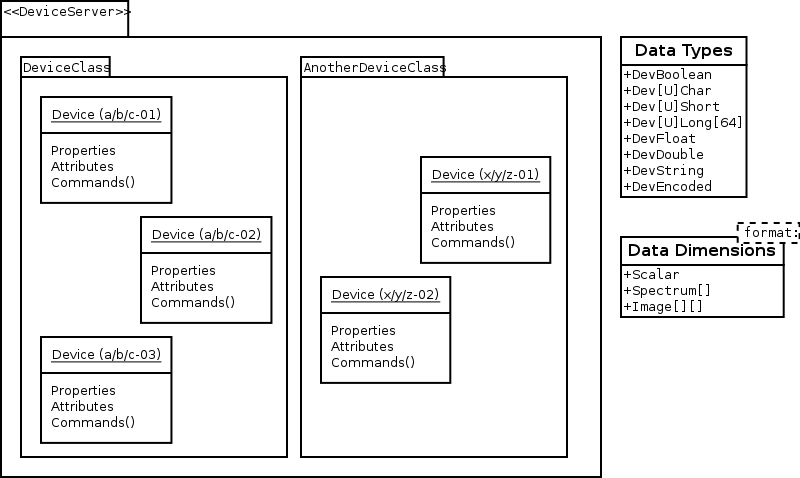
\includegraphics[width=0.7\textwidth]{imgs/tango_DeviceServer_DeviceClass_Device.png}
         \caption{\tango\, agents process structure \fixme{To be improved}} \label{fig:tangoDeviceStructure}
    }
\end{figure}

\subsection{\tango\, transparencies}

Now, with this knowledge is time to move back to the table \ref{tab:transparencies} about distributed system transparencies. As \tango\, is a software built above \corba, it is using it to deal with the degree of support of those transparencies.

The 8 transparencies shall be divided in 3 groups: the ones provided by the middleware tools, the ones that depends on the code in the agent, and the ones not present in \tango.

\paragraph{Transparencies provided by middleware:} The first group, starts with the \emph{access} transparency. It is because of the \corba\, common data types in the \emph{IDL} (Interface Definition Language) files that the data types are homogenized in a tango system. Forget if compiler set an \texttt{int} of 16 or 32 bits, a DevShort will have 16 every where and DevLong 32. Next, \emph{Location} transparency is not supported by the middleware, every search for an agent (for example, by name) will require an access to a \tango-db, that one can see it as a \emph{phone-book} of agents and this is a \emph{centralized} weak point. Any issue on the database server makes you blind in the system. Even is the agents continue working you would be unable to see it, and the performance of the system decays when agents are trying to communicate with other agents.

\paragraph{Transparencies provided by agent developer:} The second group of transparencies are the ones that depends on developer sensitivities. In this case, there is no supervision about if it supports it or not. The first transparency that depends on the developer of an specific \emph{DeviceServer} is the \emph{concurrency}. The way the specific devices does the job when an operation is requested to them, is only managed by the agent developer. From the code in \emph{SourceForge}, there are more examples of agents that does not support concurrency than examples to follow in a new development. This is very related with the \emph{persistence} transparency, because again, the code to access an specialised hardware is embedded in the agent code. To often a user can not distinguish a hang agent than a hanged instrument. And again this links to the \emph{failure} transparency. In my humble opinion, the issue comes from the \emph{extreme programming} philosophy, because to often, when a \emph{DeviceServer} is 
launched with the hardware not present, instead of a notification from the \emph{Device} the situation is a premature death of the agent.

\paragraph{Not supported transparencies:} And the third group are transparencies not supported at all. \emph{Migration}, \emph{relocation} and \emph{replication} are transparencies not supported by \tango. But despite a weakness it is a design choice. The agents cannot move their code from one machine to another while you use them. When a device is restarted, event in the same machine, it has lost any request you made to it. When \emph{migration} is not supported, \emph{relocation} even less. \emph{Replication} is a task to be made by humans and agents have not capabilities to decide anything about that.

\subsection{Attacks}

% \begin{itemize}
%     \item Attacks
%     \begin{itemize}
%         \item \ok{Eavesdropping: passive attack}
%         \item \ok{Men-in-the-middle}
%         \item \ok{Noise-Interruption-Poisoning: Break the public face, web site, gui, vital agent}
%         \item \ok{Spoofing: mask and/or falsify data}
%         \item \ok{Modification/Fabrication: Supplant/tampered agents (code authentication).}
%     \end{itemize}
%     \item \ok{Detection and recovery: auditor agents}
% \end{itemize}

Previous references to books in section \ref{sec:SecurityEngineering} let seen between practical attacks to a distributed system like \tango. But event this type of system have some peculiarities, there are many things that can be reused. In a widespread distributed system, the agents communication is not too different than RFID card/reader communication \cite{Santi11}. The figure \ref{fig:tangoLayout} shows an example of the agents involved in a normal operation of the Control System. For example, in the centre there is a representation of an agent in the distributed system in charge of the alarms. This is a key device in charge to do the monotonous task of check that everything is running as expected. This is a good example because this must be able to talk with every one that is being monitored.

First type of attacks to any system, are the passive \emph{Eavesdropping}. An attacker can do almost the same than this agent in charge of the alarms but not to advice about problems, but something else like record private information, like can be data from a scientific experiment or industrial secrets.

There are other type of attacks that passes the line of the observation and starts to introduce actions to the system, and that is why they are called \emph{active}. There are many different ways to do this tasks. The most known is the \emph{Men-in-the-middle}, with good skills when the two participants to the communication, and because they do not know each other (no authentication), have the communication bridged by some one else in the middle that is repeating the communication from one to the other and all the information is accessible to this Eavesdropper. This attack is just half a way between active and passive, but often is combined with the other type of active attacks.

The active attacks can be splitted in three main categories: avoid the information transmission, avoid the reception, modify the transmitted information. For the first case, adding enough noise to the communication channel you can block the transmission of data from RFIDs and in this case you may not distinguish from where there are not cards. In a distributed control system the situation is different because, the environment are better known. The disappearance of a device will be perceived. But there are other degrees of this noise attack, perhaps with only poisoning the information the attack can reach the goal. Imagine a device that is raising an alarm, but the attacker is interrupting this. Even further the attacker can \emph{spoof} (modify or send an old message with a new time stamp) the data and the receivers still think that everything is going well. Still more beyond, the alarm device can be completely supplanted or tampered and build information from inside the system like one more of the agents.

It is mandatory in any system that likes to practice security, not only to have the necessary tools to protect itself to the attacks, but the tools to detect if something has crossed the barriers. As was been mention about perfect security in \ref{sec:SecurityEngineering}, do never have an \emph{ego} that makes you thing no one can cross the defences. But detection is nothing if there is not recovery. Never forget the social engineering against supervisors, and left the first line of this work to \emph{auditor agents} that, in case of detection, can start the fight and the humans get notice to monitorise what is happening.

\begin{figure}[h]
    \centering{
         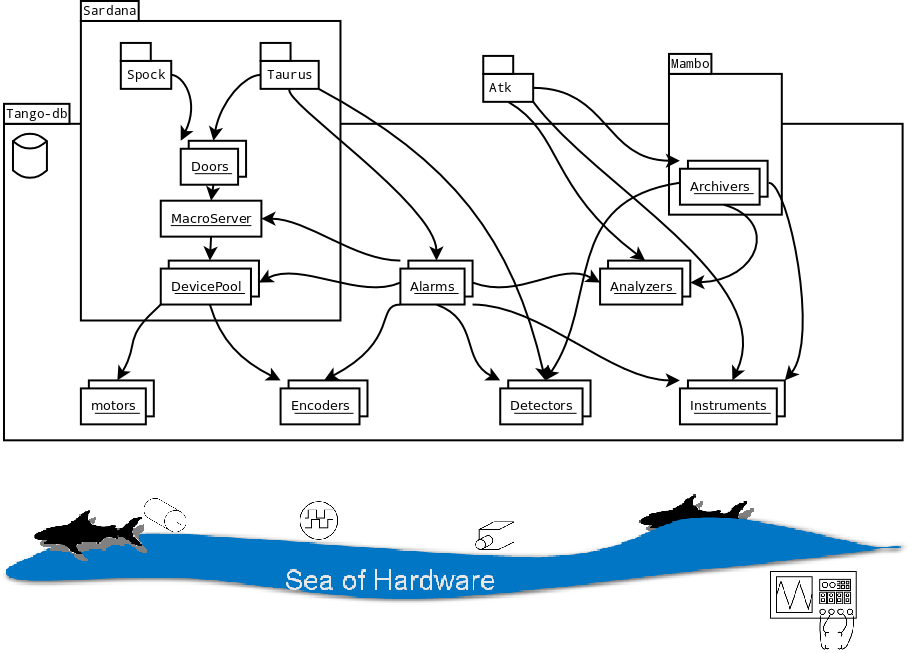
\includegraphics[width=0.75\textwidth]{imgs/tango_layout.png}
         \caption{\tango\, schematic layout \fixme{To be improved significantly}} \label{fig:tangoLayout}
    }
\end{figure}

%%%%%%%%%%%%%%%%%%%
\section{Solutions}\label{sec:solutions}

Although in security engineering section \ref{sec:SecurityEngineering} the pointed scenarios can lead to think in solutions like \emph{fingerprint readers} or \emph{iris scanners}, the purpose of this paper focus on agents interrelations inside networked computers, and is not about human access to the system.

What \tango\, needs as final product that introduces security, is to add to the URI naming an '{\tt s}' of secure in the protocol name like web had with ``\emph{http}{\tt s}'' or many other service like ``\emph{smtp}{\tt s}'', ``\emph{imap}{\tt s}'' or if need be, how the ``{\tt ssh}'' has replaced the ``\emph{telnet}''. There is not enough activating the {\tt OpenSSL} flag in the \omniorb\, compilation, there are levels of abstraction above \corba\, that must be covered.

Another fact has been mention in section \ref{sec:SecurityEngineering} and it is about the issue that any agent can not be trusted if the machine where this agent runs can not be trusted. It does not have any sense to trust in an agent that is carrying a secret key that may have been compromised during an execution inside a machine that is out of our trust ring.

Once said this points, it is time to go inside of the proposed solutions for \tango. Here we have two main solutions in the next subsections to complain with the basic principles of \emph{information security} (see table \ref{tab:infosec} in section \ref{sec:InfoSec}), followed by two introductions to advance solutions.

\subsection{Use of \emph{Elliptic curves} for authentication and public key encryption}\label{sec:authentication}

%     \begin{itemize}
%         %\item Important: agents can only be authenticated if they run on trusted machines. Other ways is useless that an agent carries a private key if it can be saw by a compromised machine.
%         %\item Because the mix with computationally powerful hardware, living with embedded systems, the solution must follow the most restrictive, to also follow the \emph{access} transparency of a distributed system.
%         %\item Following section \ref{sec:securityLevels}, inside an institution some sets of different curves distinguishing the level by the curve size but also different curves of the same size to separate systems with the same level of secrecy but isolate them in cryptoanalysis. Isogeny volcanoes \cite{secRickShareECs}. Together with the contribution work of \cite{JValera11}, \cite{Ramiro05}, \cite{Rosana11}.
%         %\item Capability to reset a curve setup on any of those secrecy levels and the feature to have different setups between different subsystems to have separated environments between them.
%         %\item Standards about elliptic curves; International \cite{rfc6637}, \cite{rfc4492} (Updated by \cite{rfc5246} and this one by \cite{rfc5746}, \cite{rfc5878} and \cite{rfc6176}), \cite{sec1}, \cite{sec2}, USA: \cite{P1363}, \cite{X9.62-1998}, German: \cite{brainpool},\cite{BSI_TR-03111}, Russian: \cite{GOSTR341001}
%         %\item \todo{\tango-db as the base for PKI (\emph{Public Key Infrastructure} and CA (\emph{Certificate Authority)}}
%     \end{itemize}

The \tango\, DCS runs its agents in very different kinds of hardware. It is possible that an agent runs in a huge server with more resources that it could even use, and the same agent later on is moved to an embedded board where the resources are extremely limited. Or perhaps the user interface runs in a good workstation with genuine resources, and there must not be differences between device running in big or small machines. Remember this is a requirement for distributed systems transparencies (focus in \emph{access} transparency, see section \ref{sec:DistrSys} table \ref{tab:transparencies} and specifically about \tango\, in section \ref{sec:characteristics}, these are tools that the \emph{middleware} must provide).

Elliptic curves are a very good tool to be helpful with this scenarios where embedded system coexist with others. But there is another feature of the elliptic curves that can be useful here. Remember in the \emph{security levels} (section \ref{sec:securityLevels}) where the idea of different systems that shares the same levels should be isolated between them, and this solutions is helping this requirement, because with a different elliptic curve per subsystem, the cryptanalysis on each is different even if they are defined over  a finite field of the same size (even when they share the same prime).

Nowadays there is a big discussion over this possibility of the curves use. The beginning of the standardisation there where two tendencies: allow any curve or restrict the number of curves. Focussing on the ANSI X9.62 recommendations \cite{X9.62-1998}, not only restrict the set of curves is bad, but too many keys sharing a curve are a thread by itself. For this purpose the use of the NIST curves is not enough (they have been published in 2000 with in the annex 6 for the FIPS PUB186-2 updated in a third version \cite{NIST186-3} in 2009) even they come from a bit bigger list from \cite{sec2}. The standard for \emph{OpenPGP messages} \cite{rfc6637} restricts even more this set to only 3 curves for all the world over 3 security levels on the standard. When in another hand, the standard for \emph{TLS} with curves \cite{rfc4492} allows any curve from certain formulations of the curves over \ensuremath{\mathbb{F}_{p}} and \ensuremath{\mathbb{F}_{2^m}}.

The final solution must not restrict to a set of curves. Even if a new set of curves is added, like can be the \cite{brainpool}, it will never be enough for a world wide use. A smaller restriction of a set of curves described in a certain way like is the Weierstrass Reduced From is potentially also an issue if new sets of good curves are discovered like the ones proposed in \cite{cryptoeprint:2013:647} (Montgomery and Edwards formulations).

In fact, what can help to follow the recommendations from the the ANSI X9.62 is to have a public auditable algorithm to allow each one to generate its own curve. Perhaps, in case this is a computationally expensive cost, all the keys within a subsystem of one particular security level, should have its own curve. This is a feature that is not easy to implement for solutions like \emph{OpenPGP}, but is an environment where the public key infrastructure is build from scratch this is a feature that can be included.

On this public auditable algorithm, there is work on going \cite{secRickShareECs} where is proposed solutions based on \emph{Complex multiplication} or in elliptic curve \emph{isogenies}. This work has been based in previous development of \cite{Ramiro05}, \cite{Rostovtsev06public} \cite{Rosana11}, and \cite{JValera11}. From this two possible solutions, one has an extra feature, because from the idea of a public key cryptosystem using isogenies \cite{Rostovtsev06public} would be possible to introduce a new operation that any other system can not do: the \emph{cryptosystem reset}. This feature could allow the system to renew the elliptic curve in use, by a newer one with the same size but where if there is any attack ongoing on the first curve, the cost to \emph{migrate} the attack from one curve to the other will be bigger than start the attack on the second from scratch.

As mention, the \emph{Public Key Infrastructure} (short for PKI) and the \emph{Certificate Authority)} (short of CA) has to be designed from scratch to be inserted in the \tango\, middleware. And this is a great advantage because this can save many of the design issues where the current infrastructure have limitations. It is a great opportunity to have nothing that forces backward compatibility on this point, but is a great responsibility because each decision on this matter will affect the later evolution. As \tango\, has, and will probably continue having, the \tango-db, this PKI can use it. But if someday, \tango\, does one step further in distribution, a hard link on that would be a lace shoe pinches.

\todo{Figure about how an agent can be identified, authenticated and authorized.}


\subsection{Lightweight symmetric and/or stream ciphers}\label{sec:encryption}

%     \begin{itemize}
%         %\item Adapt the symmetric algorithms to manage the block size in the same size of the data block. If with symmetric systems the data block is smaller than the cipher block, there is an expansion in the data transmission from the insecure option.
%         %\begin{itemize}
%         %    %\item Adapt the Rijndael \cite{gRijndael} (AES contest \cite{AES-FIPS} and the book \cite{Daemen:2002:DR:560131})
%         %    %\item key size must be related with the security levels (section \ref{sec:securityLevels}) and this also has relation with the number of rounds
%         %\end{itemize}
%         %\item Possibilities of the AESWrap \cite{rfc3394}
%         \item stream ciphers: non block size limited for event transmission
%         \begin{itemize}
%             \item Key derivation Funtions as PRGs for stream ciphers
%             \item Rabbit \cite{rfc4503}
%             \item \emph{Secret splitting} for multicasting information.
%         \end{itemize}
%     \end{itemize}

Once a device is authenticated and there is a secure channel using asymmetric encryption, this can be used to exchange session key when an attribute likes to be accessed. This paper proposes two main ways: symmetric algorithms and/or stream ciphers. Both have \emph{pros and cons} and a hybrid system would support both and use the best of them depending on the situation. The key agreement should also agreed how the later communication will be.

The constrains to select one way or the other must be the flux of data. The needs are very different when the transmission means a boolean subscribed that changes every few milliseconds, or if the transmission is a detector image of 6 mega-pixels, where each pixel is a \emph{DevLong} ($32$ bit size), generated in the order of the hundreds of milliseconds.

\paragraph{Symmetric algorithms:} The first of the solutions proposed for the information transmission is the use of lightweight symmetric algorithms. An important feature for this is the possibility to adapt the sizes of the blocks to be used, together with the encryption modes.

One of the most used algorithms for symmetric encryption is the \emph{Rijndael}. This was the winner of the \emph{Advanced Encryption Standard} (short of AES) \cite{AES-FIPS} that replaces the \emph{DES} algorithm. There is a book \cite{Daemen:2002:DR:560131} from the algorithm authors that explains very well the mathematics behind this algorithm. The original algorithm supports a block size of 128 bits and 5 key sizes (128, 160, 192, 224 and 256 bits) but when it was standardised, there where only used 3 of them (128, 192 and 256). But based on the mathematics behind it is possible to fine tune both sizes, the block and the key. There is a work in progress on this field \cite{gRijndael} that is trying to adapt the \emph{Rijndael} to be used as lightweight symmetric and also with sizes above the originals.

In the context of this paper, it is important to have smaller block sizes because the attribute types (section \ref{sec:characteristics}) are smaller than the basic block size and using directly the AES will at least duplicate the information to transfer for each value.

About the other block size change, the key size, can be useful the feature to have much more key sizes in order to have it in correspondence with the related security levels mention in section \ref{sec:securityLevels}. The paper mentioned there \cite{lenstrauniversal13} about the key sizes remarks also that it is mandatory to have correspondence between the three elements in a pack of security: public key, symmetric and hash\footnote{In this paper are not included the hash algorithms as like as the symmetric algorithms are due to an scope reason, but with them it happens a similar thing than with the \emph{Rijndael}.} sizes. This sizes must be selected with utmost case, because the weakest is our incoming invitation to the attacks.

\todo{Set up a figure with an input key with size depending on the security level, \& block size depending on the size of the data to encrypt.}

\todo{In the case of \emph{scalar} dimension ($0D$) perhaps a data block a bit bigger than the data can store a \emph{padding} for integrity}

\todo{In arrays of data, like \emph{spectrum} and \emph{image} dimensions ($1D$ \& $2D$), block size can match the size of the data type and use \emph{block cipher modes}:}

\begin{itemize}
    \item ECB: it has not a good randomness.
    \item CBC: requires padding and encryption is not parallelizable. 
    \item PCBC: not parallelizable.
    \item CFB: encryption not parallelizable.
    \item OFB: not parallelizable.
    \item[!!] CTR: turns a block cipher into a stream cipher. parallelizable and not requires a padding.
\end{itemize}

\todo{Figure with the CTR mode for arrays.}

\paragraph{Stream ciphers:} There is another tool for the information transmission to be explored. This has the advantage of non block size limitation. One can see it as one particular case of symmetric systems. As it is a very often system used for broadcasting information, it is a candidate for the multicasting feature of the events emission using the \zmq. There is a field in cryptology, called \emph{secret splitting} that focus in this multicast feature.

Basically a stream cipher is a \emph{Pseudo Random Generator} (short for PRG) and is very tricky because the key size choice is not the only restriction on it, there is also the live time of the key. The source of this systems are \emph{Key Derivation Funtion}s (short for KDF) used as PRGs to {\tt xor} the key flow with the data flow. As this is almost a \emph{One Time Pad} (short for OTP) the system can be considered a \emph{perfect secrecy} as define by \emph{Shannon} in \cite{shannon-comTheorySecSys}. But do not forget that is almost OTP and the only way to maintain it secure is to renew the key before the KDF can start to produce repeated sequences.

\todo{Many of the stream ciphers shows a limitation on the key size. Like {\tt Rabbit} \cite{rfc4503} has been only designed to $128$bits (with and initialisation vector $IV$ of $64$bits, or {\tt Chacha} \cite{bernstein2008chacha} has $256$bits for the key.}

\todo{To overcome the key size limitation, it can be good to use the KDF of the AESWrap \cite{rfc3394} to be a bit flow generator (This AESWrap is an extension to the AES, like the 3DES was to the DES).}

\subsection{Further advanced solutions}\label{sec:advancedSolutions}

Apart from the two solutions to introduce security in the communication between agent in a Distributed Control System like \tango, other features can be developed inside this system to provide security under other aspects of its operation. First of all will be highlighted the solution to introduce cryptography in the \tango-db, but one should not forget that this is a centralized element in a distributed system that, more than think in secure it, could be better to think in secure distributed alternatives.

There is another advanced solution proposed, basically thinking in one of the scenarios mention in section \ref{sec:SecurityEngineering} (the bank remember the bank scenario). A desired feature for a Distributed Control System would be to have integrated with in the middleware the possibility to have \emph{command authorization}, like can be to have the \emph{acknowledge} from 3 users (or even agents) from a set of many more.

\subsubsection{Cryptography for the database}\label{sec:Database}

The \tango-db, as has been described in section \ref{sec:characteristics}, is used mainly for two functions: a \emph{phone-book} to locate the agents in the system and for the permanent storage of the \emph{properties} that are, at the end, the configurations for the agents when they start running. Now a days there is no authentication at all in this part of the system, while it is true that the \mysql database access can be password protected, the middleware access to this database allows anyone within the system to, not only query, but also modify this database.

A desirable feature can be to provide this database with access authentication once the agents (and the users) have this system proposed in section \ref{sec:authentication}. But what about the contents? The solutions about encryption provided in section \ref{sec:encryption} are not a choice for database contents. There is a field in cryptology called \emph{Homomorphic encryption} (also known as \emph{Ordered cryptography}) that explores this possibility.

    \begin{itemize}
        %\item Permanent storage in a database, where there is no authentication of who is doing an operation.
        \item Homomorphic encryption:
        \begin{itemize}
            \item ``Fully homomorphic encryption using ideal lattices'' \cite{Gentry:2009:FHE:1536414.1536440}
            \item ``Fully Homomorphic Encryption with Relatively Small Key and Ciphertext Sizes''\cite{SmartVecauteren10}
            \item ``Can homomorphic encryption be practical?'' \cite{Naehrig:2011:HEP:2046660.2046682}
            \item ``Faster fully homomorphic encryption'' \cite{stehle2010faster}
            \item ``Private database queries using somewhat homomorphic encryption'' \cite{iacr422}: Ordered cryptography.
            \item ``Homomorphic Encryption: Theory \& Applications'' \cite{Jaydip2013}
        \end{itemize}
%         \item Searchable symmetric encryption
%         \begin{itemize}
%             \item 
%         \end{itemize}

        %http://outsourcedbits.org/2013/10/06/how-to-search-on-encrypted-data-part-1/
    \end{itemize}

\subsubsection{Command authorizations}\label{sec:secretSharing}

As mention in the scenario of a bank in section \ref{sec:SecurityEngineering}, a desired feature can be the dilute the authorization with more than one controller (agent or human). This kind of solutions can come from \emph{Secret Sharing} solutions. The secret sharing schemas are based on the primitive that there are $n$ participants and from them are required $k$ to access one specific secret. This is called \emph{(k,n)-threshold} schemas, and the interesting point is that the $k$ required should not be established in advance. Any combination of $k$ from the $n$ participants will grant access to the secret, and this secret can be used for anything, for example in this case authorise an operation.

\begin{itemize}
    \item \todo{reference to secret sharing}
\end{itemize}

    
%%%%%%%%%%%%%%%%%%%
\section{Conclusions}\label{sec:conclusions}

% \begin{itemize}
%     \item Add security to a DCS like \tango\, is not to simply add the flag to \omniorb\, compilation to use {\tt openssl}. Much more work must be done in the level of the \emph{middleware} as: \emph{identify}, \emph{authenticate} and \emph{authorise}. And this together with countermeasures when necessary.
%     \item \tango-db is a weak point in the DCS. Explore tools like {\tt UPnP} protocols to discover elements in the system.
%     \item Debug on the fly will be harder due to the countermeasures to tampering. Code testing procedures required.
%     \item Many more ideas can be taken from this paper as \emph{further work}.
% \end{itemize}

As has been mention at the beginning, introduce security to a Control System like \tango\, is not as simple as activate the flag to \omniorb\, to compile it using {\tt openssl}. With this the middleware will have a very interesting access to many primitives in this free software, but the schemas where these primitives some higher level protocols must be developed and implemented for bidirectional authentication of the communication actors (always thinking that they would be agents or users). In the case of the data transmission, the {\tt openssl} would be not enough. Some algorithms must be gently modified from the standards, to adapt to the specific needs of this case. And must insist on the idea of this finely adjustments because it can break the maths behind, and there must be a consciousness revision to avoid side channel attacks.

After the basics for introduce security on this system, not forget that other elements can be weak (and the weaker will mean the attack). In this text some issues with the \tango-db has been pointed, but would be good to explore other distributed solutions like the {\tt UPnP} protocols to discover elements in the system and the permanent storage.

This has been only a start, highlighting what has been already isolated as possible thread and pointed to some solutions. But the fly to this destination will be long. Also this solutions will require a mind change on the development because, something like \emph{debug on the fly} will be harder when the system have countermeasures against tampering. Code testing procedures will be required to the order of satellite navigation systems or similar.

\bibliographystyle{ieeetr}
\bibliography{../bibtex/sblanch.bib,../bibtex/books.bib,../bibtex/standards.bib,../bibtex/rfc.bib,../bibtex/tango.bib,../bibtex/crypto.bib,../bibtex/ecc.bib,../bibtex/isogeny.bib,../bibtex/symmetrics.bib,../bibtex/rijndael.bib,../bibtex/stream.bib,../bibtex/homomorphic.bib}

\end{document}
